\documentclass[a4paper,11pt,openany]{book}
\usepackage[utf8]{inputenc}
\usepackage[left=2.54cm,top=2.54cm,right=2.54cm,bottom=2.54cm]{geometry}
\usepackage[spanish]{babel}
\usepackage{amsmath}
\usepackage{amsfonts}
\usepackage{amssymb}
\usepackage{graphicx}
\usepackage{color}
\usepackage[usenames,dvipsnames]{xcolor}
\usepackage{pifont}
\usepackage{marvosym}
\newtheorem{teo}{Teorema}
\newtheorem{ejemplo}{Ejemplo}
\newtheorem{defi}{Definición}
\newtheorem{coro}{Corolario}
\newtheorem{prueba}{Prueba}
\newtheorem{exmp}{Example}[section]
\newtheorem{ejer}{Ejercicio}[section]
\def\proof{\paragraph{\textsf{Demostración.} }}
\def\endproof{\hfill $\blacksquare$ \\}
\usepackage{multirow, array} % para las tablas
\usepackage{multirow}
\usepackage{tabularx}
\usepackage{float} % para usar [H]
\usepackage{tikz}
\usepackage[all]{xy}
\usepackage{cancel}
\usetikzlibrary{positioning}
\usepackage{enumitem}
\newcommand*{\itembolasazules}[1]{% bolas 3D
\footnotesize\protect\tikz[baseline=-3pt]%
\protect\node[scale=.7, circle, shade, ball
color=green]{\color{white}\Large\bf#1};}
\usepackage{tcolorbox} 
\tcbuselibrary{listingsutf8}
\newtcolorbox[auto counter,number within=section]{example}[2][]
{colback=green!5!white,colframe=green!75!black,fonttitle=\bfseries, title=Ejercicio~\thetcbcounter: #2,#1}
\usepackage{background}
\backgroundsetup{
placement=center,
angle=0,
scale=1.1,
contents= {{
\includegraphics{HojaCuadriculada.png}}}
}
 
 
\begin{document}
\begin{titlepage}
 
\begin{center}
\vspace*{-1in}
\begin{figure}[htb]
\begin{center}

\includegraphics[width=7cm]{ETITC.png}
\end{center}
\end{figure}
 
 
{\sc \huge Escuela Tecnológica Instituto Técnico Central (ETITC)}\\
\vspace*{0.15in}
Facultad de sistemas\\
\vspace*{0.6in}
\begin{Large}
\textbf{Taller 5 : Integrales Complejas y Teorema de Cauchy - Goursat.} \\
\textbf{Matem{\'a}ticas Especiales}\\
\end{Large}
\vspace*{0.3in}
\begin{large}
{\bf Autores} \\
 
\ 
 
Sergio Alejandro Enrrique Caballero Leon\\ 
Johan Alejandro Sogamoso Camacho \\
David Andrés Valero Vanegas \\
\end{large}
\vspace*{0.3in}
 
\end{center}
 
\begin{center}
{\bf Presentado a:} \\
 
\ 
 
Carlos Romero \\
 
\
 
Bogot{\'a}, Noviembre de 2022.
\end{center}
 
\end{titlepage}

\newpage

\definecolor{ao(english)}{rgb}{0.0, 0.5, 0.0}

\graphicspath{ {images/} }

\begin{center}
\textbf{Integrales Complejas}
\end{center}

Evalue las sigientes integrales a lo largo del controno indicado en cada caso.\\

\textcolor{ao(english)}{(\,1\,)} $\bf{\displaystyle\int\limits_{C}\,(5\,-\,z^{2}\,+\,2\,z)\,dz}$.

\begin{center}
     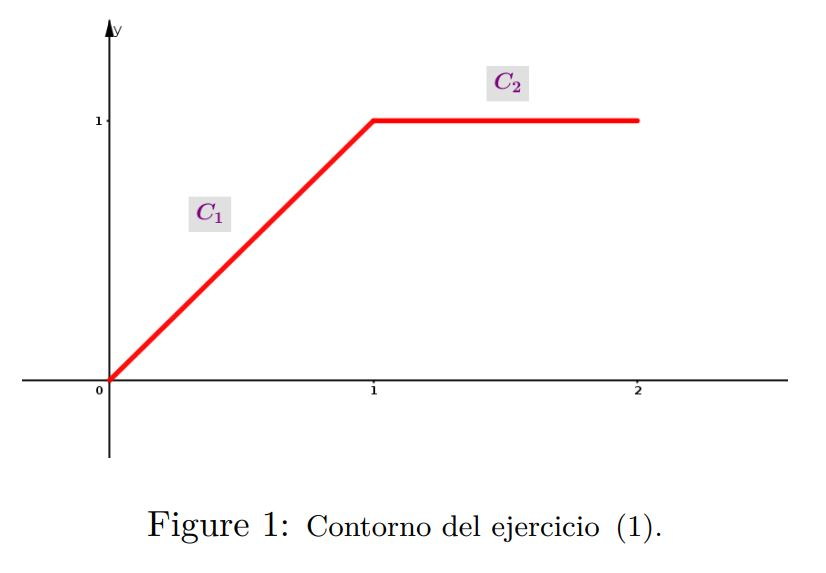
\includegraphics[width=10cm]{figura-1.JPG}
\end{center}


El contorno está dado por:\\

$$C_{1} \quad\iff\quad x\,=\,y,\,0\leq\,x\,\leq,\,y\,=\,0$$

$$C_{2} \quad\iff\quad 1\leq\,x\,\leq\,2,\,y\,=\,1$$

$\bf{\displaystyle\int\limits_{C_{1}}\,f(z)\,dz}$.\\

\textcolor{ao(english)}{\ding{47}\,Paso 1:} Escribir $z$ en terminos del parámetro.

$$z\,=\,x\,+\,i\,y \qquad\iff\qquad z\,=\,x\,+\,i\,x$$

\textcolor{ao(english)}{\ding{47}\,Paso 2:} Escribir $dz$ en terminos del parámetro.

$$\dfrac{dz}{dx}\,=\,1\,+\,i \quad\iff\quad dz\,=\,(1\,+\,i)\,dx$$

\textcolor{ao(english)}{\ding{47}\,Paso 3:} Escribir $f\,(z)$ en terminos del parámetro.

$$f\,(z)\,=\,(5\,-\,z^{2}\,+\,2\,z)\,=\,5\,-\,(x\,+\,i\,x)^{2}\,+\,2\,(x\,+\,i\,x)$$

\textcolor{ao(english)}{\ding{47}\,Paso 4:} Escribir la integral.

$$\bf{\displaystyle\int\limits_{C_{1}}\,f(z)\,dz}\,=\,\displaystyle\int_{0}^{1}\,[5\,-\,(x\,+\,i\,x)^{2}\,+\,2\,(x\,+\,i\,x)]\,(1\,+\,i)\,dx$$

$$=\,(1\,+\,i)\,\displaystyle\int_{0}^{1}\,[5\,-\,(x\,+\,i\,x)^{2}\,+\,2\,(x\,+\,i\,x)]\,dx$$

$$=\,(1\,+\,i)\,\displaystyle\int_{0}^{1}\,[5\,-\,(x^{2}\,+\,2\,x^{2}\,i\,-\,x^{2})\,+\,2\,x\,+\,2\,x\,i)]\,dx$$

$$=\,(1\,+\,i)\,\displaystyle\int_{0}^{1}\,[5\,-\,2\,x^{2}\,i\,+\,2\,x\,+\,2\,x\,i)]\,dx$$

$$=\,(1\,+\,i)\,\left(5\,x\,-\dfrac{2\,x^{3}\,i}{3}\,+\,\dfrac{2\,x^{2}}{2}+\,\dfrac{2\,x^{2}\,i}{2}\bigg|_{0}^{1}\,\right)$$

$$=\,(1\,+\,i)\,\left(5\,x\,-\dfrac{2\,i}{3}\,+\,1\,+\,\dfrac{3\,i}{3}\bigg|_{0}^{1}\,\right)$$

$$=\,(1\,+\,i)\,\left(6\,+\,\dfrac{i}{3}\right)$$

$$=\,6\,+\,\dfrac{i}{3}\,+\,6\,i\,-\,\dfrac{1}{3} \qquad=\qquad\,\dfrac{17}{3}\,+\,\dfrac{19\,i}{3}$$

$\bf{\displaystyle\int\limits_{C_{2}}\,f(z)\,dz}$.\\

\textcolor{ao(english)}{\ding{47}\,Paso 1:} Escribir $z$ en terminos del parámetro.

$$z\,=\,x\,+\,i\,y \qquad\iff\qquad z\,=\,x\,+\,i$$

\textcolor{ao(english)}{\ding{47}\,Paso 2:} Escribir $dz$ en terminos del parámetro.

$$\dfrac{dz}{dx}\,=\,1 \quad\iff\quad dz\,=\,dx$$

\textcolor{ao(english)}{\ding{47}\,Paso 3:} Escribir $f\,(z)$ en terminos del parámetro.

$$f\,(z)\,=\,(5\,-\,z^{2}\,+\,2\,z)\,=\,5\,-\,(x\,+\,i)^{2}\,+\,2\,(x\,+\,i)$$

\textcolor{ao(english)}{\ding{47}\,Paso 4:} Escribir la integral.

$$\bf{\displaystyle\int\limits_{C_{2}}\,f(z)\,dz}\,=\,\displaystyle\int_{1}^{2}\,[5\,-\,(x\,+\,i)^{2}\,+\,2\,(x\,+\,i)]\,dx$$

$$=\,\displaystyle\int_{1}^{2}\,[5\,-\,(x^{2}\,+\,2\,x\,i\,-\,1)\,+\,2\,x\,+\,2\,i)]\,dx$$

$$=\,\displaystyle\int_{1}^{2}\,[5\,-\,x^{2}\,-\,2\,x\,i\,+\,1\,+\,2\,x\,+\,2\,i)]\,dx$$

$$=\,\left(6\,x\,-\dfrac{x^{3}}{3}\,-\,\dfrac{2\,x^{2}\,i}{2}+\,\dfrac{2\,x^{2}}{2}\,+\,2\,x\,i\,\right)\bigg|_{1}^{2}$$

$$=\,\left(12\,-\dfrac{8}{3}\,-\,4\,i\,+\,4\,+\,4\,i\,\right)\,-\,\left(6\,-\dfrac{1}{3}\,-\,i\,+\,1\,+\,2\,i\right)$$

$$=\,12\,-\dfrac{8}{3}\,-\,4\,i\,+\,4\,+\,4\,i\,-\,6\,+\dfrac{1}{3}\,+\,i\,-\,1\,-\,2\,i$$

$$=\,9\,-\,\dfrac{8}{3}\,-\,3\,i\,+\,\dfrac{1}{3} \qquad=\qquad\,\dfrac{20}{3}\,-\,i$$

$$\bf{\displaystyle\int\limits_{C}\,=\,\displaystyle\int\limits_{C_{1}}\,+\,\displaystyle\int\limits_{C_{2}}\,=\,\dfrac{17}{3}\,+\,\dfrac{19\,i}{3}\,+\,\dfrac{20}{3}\,-\,i\,=\,\dfrac{37}{3}\,+\,\dfrac{16\,i}{3}}$$



\textcolor{ao(english)}{(\,2\,)} $\bf{\displaystyle\int\limits_{C}\,(2\,\overline{z}\,-\,z)\,dz}$, \qquad donde \qquad $C$ es $x\,=\,-\,t \quad;\quad y\,=\,t^{2}\,+\,2 \quad;\quad 0\,\leq\,t\,\leq\,2$.

\textcolor{ao(english)}{(\,3\,)} $\bf{\displaystyle\int\limits_{C}\,z^{2}\,dz}$, \qquad donde \qquad $C$ es $z\,(t)\,=\,3\,t\,-\,2\,i\,t \quad;\quad -\,2\,\leq\,t\,\leq\,2$.\\

\textcolor{ao(english)}{\ding{47}\,Paso 1:} Escribir $z$ en terminos del parámetro.

$$z\,(t)\,=\,3\,t\,-\,2\,i\,t$$

\textcolor{ao(english)}{\ding{47}\,Paso 2:} Escribir $dz$ en terminos del parámetro.

$$\dfrac{dz}{dt}\,=\,3\,-\,2\,i \quad\iff\quad dz\,=\,(3\,-\,2\,i)\,dt$$

\textcolor{ao(english)}{\ding{47}\,Paso 3:} Escribir $f\,(z)$ en terminos del parámetro.

$$f\,(z)\,=\,z^{2}\,=\,(3\,t\,-\,2\,i\,t)^{2}\,=\,9\,t^{2}\,-\,12\,i\,t^{2}\,-\,4\,t^{2}\,=\,5\,t^{2}\,-\,12\,i\,t^{2}$$

\textcolor{ao(english)}{\ding{47}\,Paso 4:} Escribir la integral.

$$\displaystyle\int\limits_{C}\,z^{2}\,dz\,=\,\displaystyle\int_{-\,2}^{2}\,(5\,t^{2}\,-\,12\,i\,t^{2})\,(3\,-\,2\,i)\,dt\,=\,(3\,-\,2\,i)\,\displaystyle\int_{-\,2}^{2}\,(5\,t^{2}\,-\,12\,i\,t^{2})\,dt$$

$$=\,(3\,-\,2\,i)\,\left(\dfrac{5\,t^{3}}{3}\,-\,4\,i\,t^{3}\right)\bigg|_{-\,2}^{2}\,=\,(3\,-\,2\,i)\,\left[\dfrac{5(2^{3})}{3}\,-\,\dfrac{5((-\,2)^{3})}{3}\,-\,(4\,i\,(2^{3})\,-\,4\,i\,((-\,2)^{3}))\right]$$

$$=\,(3\,-\,2\,i)\,\left[\dfrac{40}{3}\,+\,\dfrac{40}{3}\,-\,(32\,i\,+\,32\,i)\right]\,=\,(3\,-\,2\,i)\,\left(\dfrac{80}{3}-\,64\,i\right)$$

$$=\,80\,-\,192\,i\,-\,\dfrac{160\,i}{3}\,-\,128\,=\,\boxed{-\,48\,-\,\dfrac{736\,i}{3}}$$

\textcolor{ao(english)}{(\,4\,)} $\bf{\displaystyle\oint\limits_{C}\,(2\,z\,-\,1)\,dz}$.

\begin{center}
     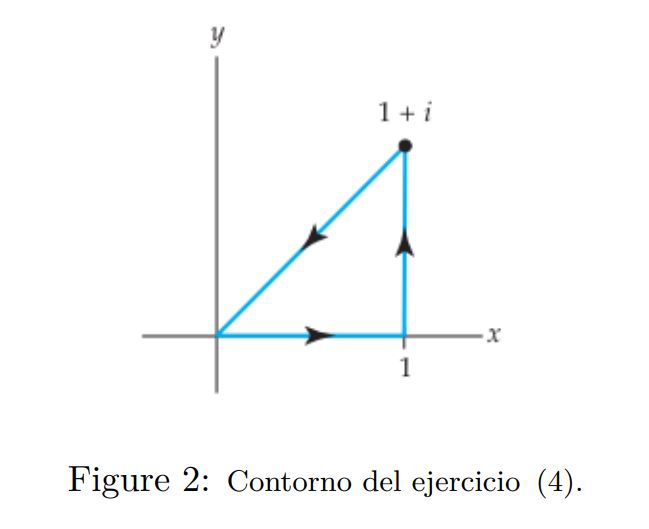
\includegraphics[width=8cm]{figura-2.JPG}
\end{center}

\begin{center}
\textbf{Teoremas de Cauchy y de Cauchy - Goursat}
\end{center}

Ejercicios \textbf{(\,5\,)} al \textbf{(\,7\,)}. Usando los procedimientos vistos en clase, \textbf{muestre y justifique} por qué $\oint_{C}\,f\,(z)\,dz\,=\,0$, donde $f$ es la función dada y $C$ es el círculo $|\,z\,|\,=\,1$, Además, dibuje el círculo en el plano complejo e indique (si lo hay), él o los puntos donde $f$ es indeterminada.\\

\textcolor{ao(english)}{(\,5\,)} $\bf{f\,(z)\,=\,z^{3}\,-\,1\,+\,3\,i}$.

\textcolor{ao(english)}{(\,6\,)} $\bf{f\,(z)\,=\,\dfrac{z}{2\,z\,+\,3}}$.

\textcolor{ao(english)}{(\,7\,)} $\bf{f\,(z)\,=\,\dfrac{e^{z}\,+\,2\,i}{(z^{2}\,-\,25)\,(z^{2}\,+\,9)}}$.\\

Ejercicios \textbf{(\,8\,)} al \textbf{(\,10\,)}. Evalúe cada integral dada a continuación usando los procedimientos vistos en clase \textbf{justificando su respuesta}. El controno se muestra en la figura o se indica en el correspondiete ejercicio.\\

\textcolor{ao(english)}{(\,8\,)} $\bf{\displaystyle\oint\limits_{C}\,\dfrac{1}{z}\,dz}$.

\begin{center}
     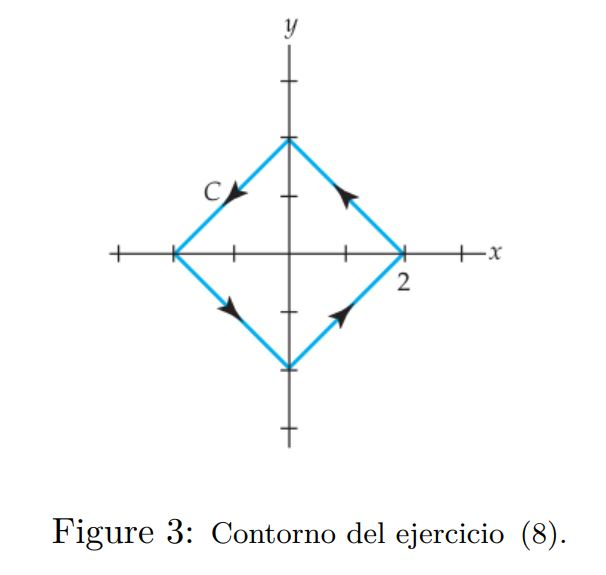
\includegraphics[width=8cm]{figura-3.JPG}
\end{center}

\textcolor{ao(english)}{(\,9\,)} $\bf{\displaystyle\oint\limits_{C}\,(z\,+\,\dfrac{1}{z})\,dz}, \qquad |\,z\,|\,=\,2$.

$$\displaystyle\oint\limits_{C}\,(z\,+\,\dfrac{1}{z})\,dz\,=\,\underbrace{\displaystyle\oint\limits_{C}\,z\,dz}_{I_{1}}\,+\,\underbrace{\displaystyle\oint\limits_{C}\,\dfrac{1}{z}\,dz}_{I_{2}}$$

\begin{tcolorbox}[colback=ao(english)!5!white,colframe=ao(english)!75!black,fonttitle=\bfseries,title=\sf $I_{1}$]

\textcolor{ao(english)}{\ding{46}} Grafica.

\begin{center}
     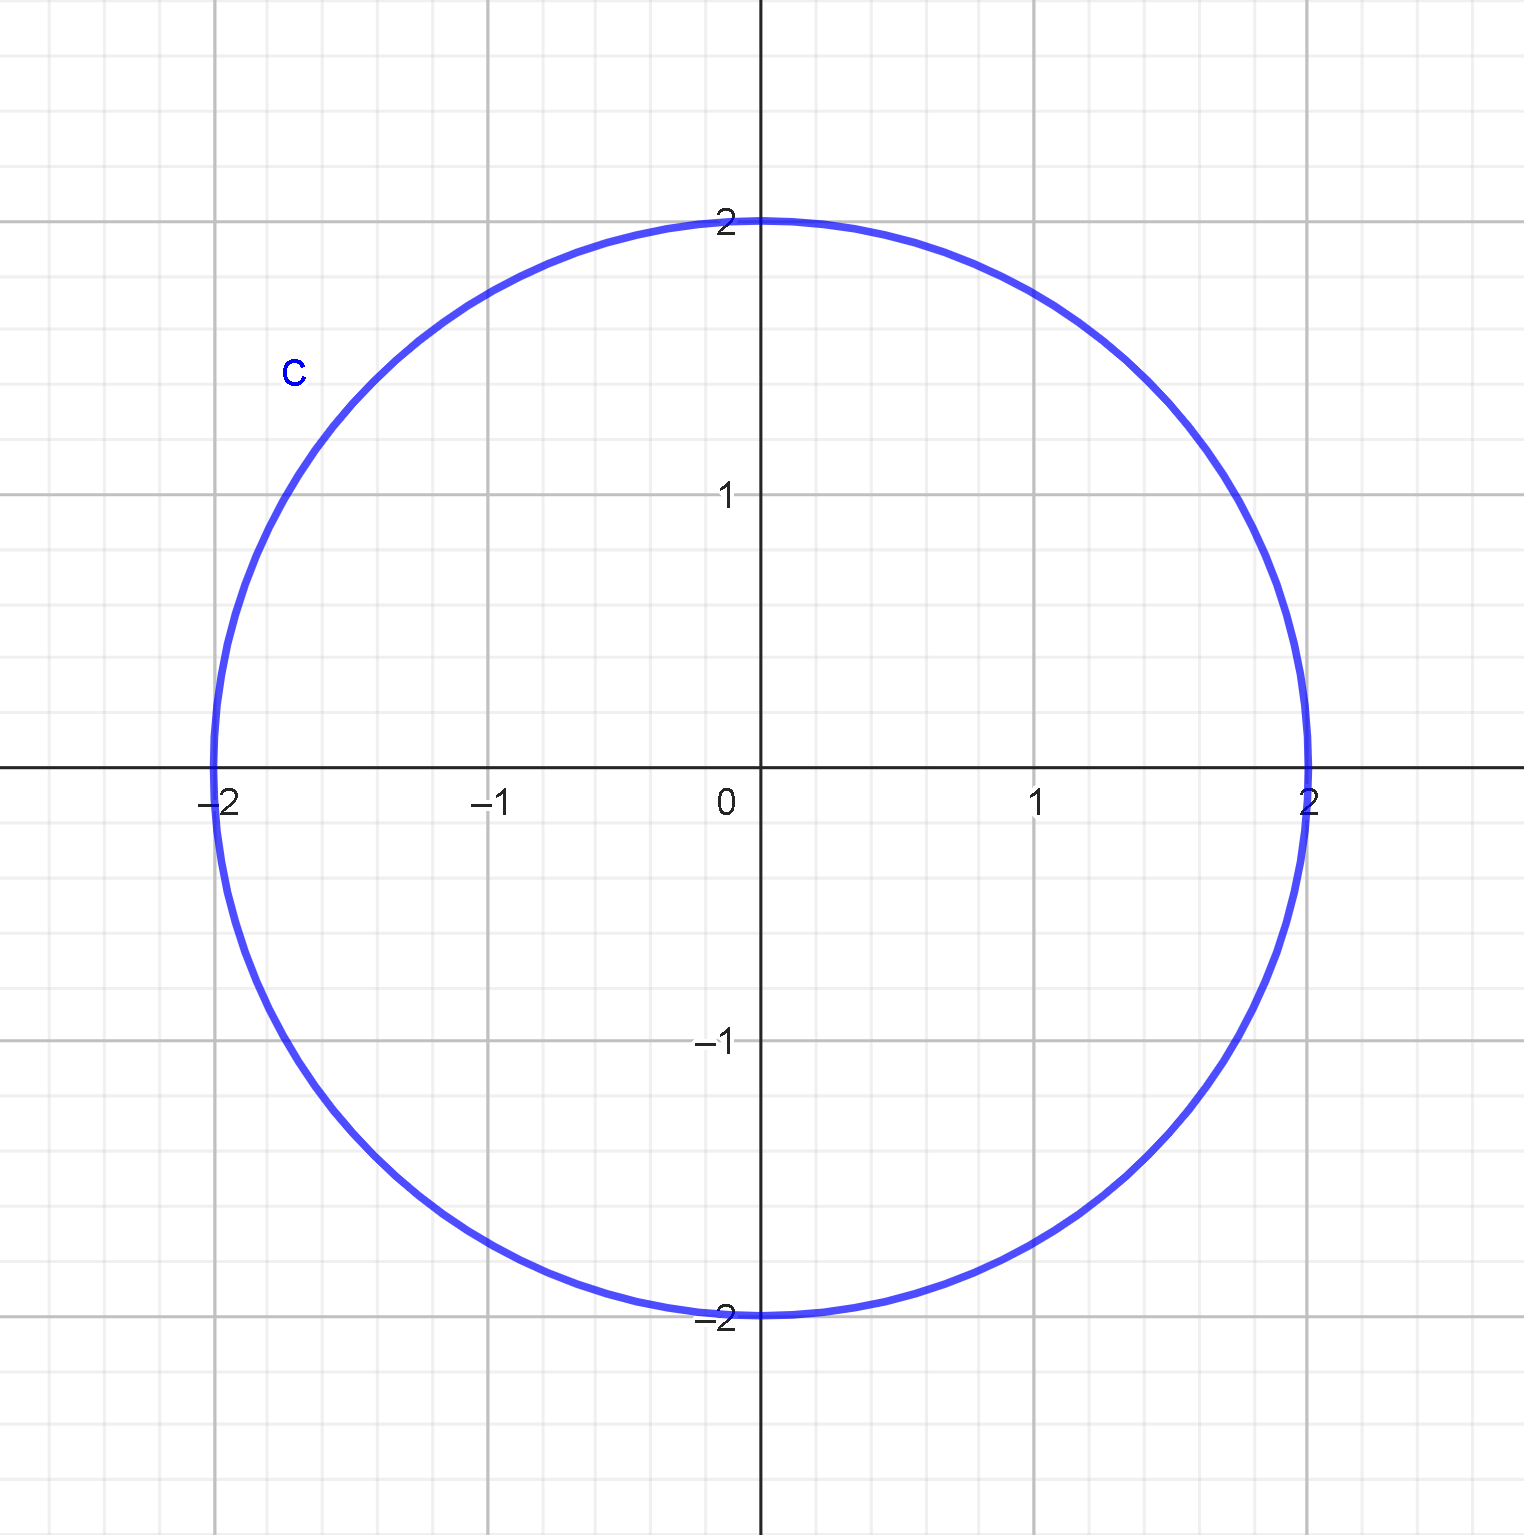
\includegraphics[width=8cm]{Gra-Ej-9-1.png}
\end{center}

\textcolor{ao(english)}{\ding{46}} Justificación.\\

$C$ es un controno cerrado simple, con $\mathnormal{Dom\,(f)}\,=\,\mathbb C$ y  es un dominio simplemente conexo. La $f\,(z)\,=\,z$ es Analitica por lo tanto el valor de esta integral es:

$$\displaystyle\oint\limits_{C}\,z\,dz\,=\,0$$

\end{tcolorbox}

\newpage

\begin{tcolorbox}[colback=ao(english)!5!white,colframe=ao(english)!75!black,fonttitle=\bfseries,title=\sf $I_{2}$]

La $f\,(z)\,=\,\dfrac{1}{z}$ es indeterminada y no esta definida en $z\,=\,0$.\\

\textcolor{ao(english)}{\ding{46}} Grafica.

\begin{center}
     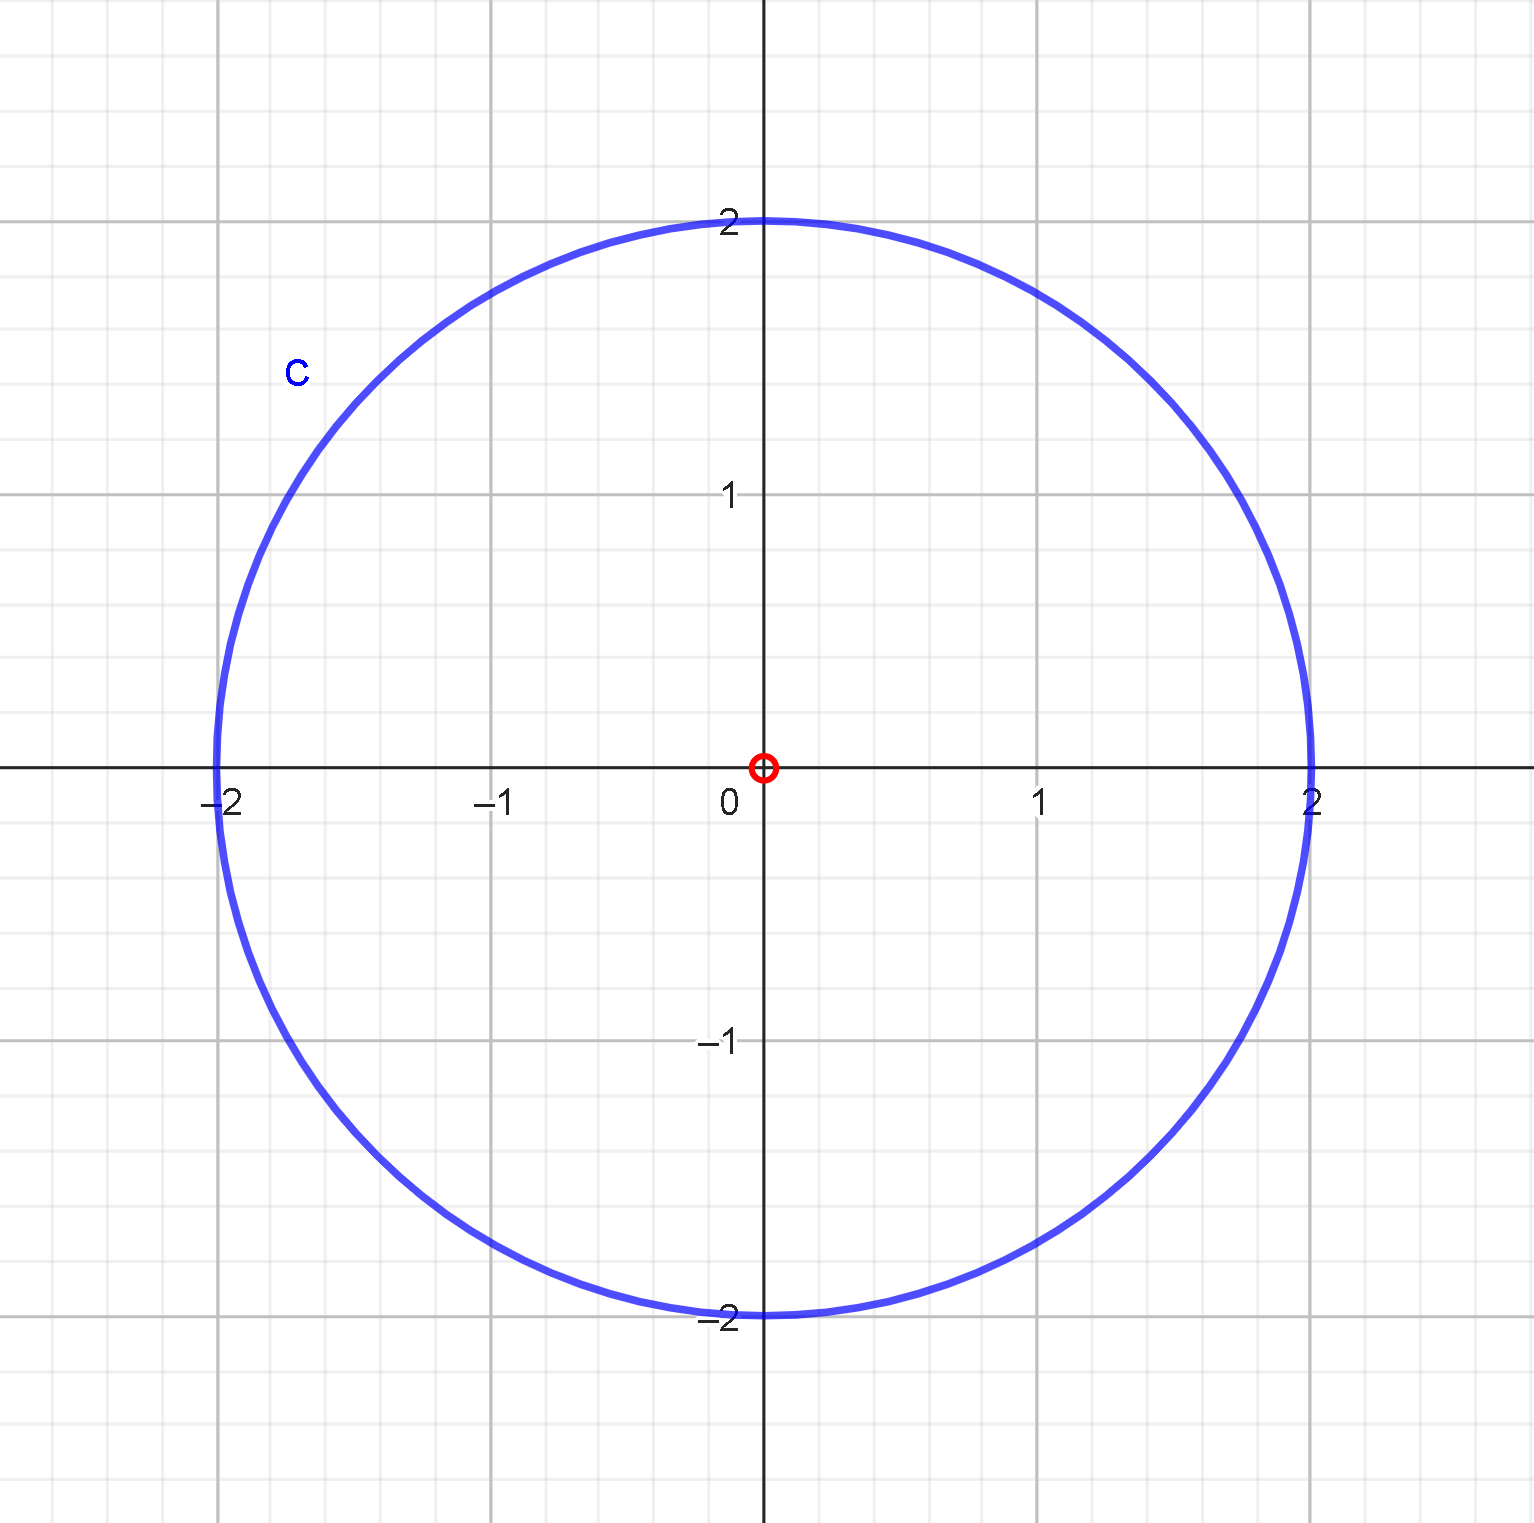
\includegraphics[width=8cm]{Gra-Ej-9-2.png}
\end{center}

\textcolor{ao(english)}{\ding{46}} Justificación.\\

$\mathnormal{Dom\,(f)}\,=\,\mathbb C\,-\,\{0\}$ es un Dominio doblemente conexo; y ya que $z\,=\,0$ está dentron del controno $C$ el valor de esta integral es:

$$\displaystyle\oint\limits_{C}\,\dfrac{1}{z}\,dz\,=\,2\,\pi\,i$$

\end{tcolorbox}

$$\displaystyle\oint\limits_{C}\,(z\,+\,\dfrac{1}{z})\,dz\,=\,0\,+\,2\,\pi\,i\,=\,2\,\pi\,i$$

\textcolor{ao(english)}{(\,10\,)} $\bf{\displaystyle\oint\limits_{C}\,\dfrac{-\,3\,z\,+\,2}{z^{2}\,-\,8\,z\,+\,12}\,dz}, \qquad (\,a\,)\,|z\,-\,5|\,=\,2 \qquad (\,b\,)\,|\,z\,|\,=\,9$.

\end{document}